%!TEX root = ../tesis_mbc.tex

\chapter{Marco teórico}
\label{ch:marco_teorico}

%%%%%%%%%%%%%%%%%%%%%%%%%%%%%%%%%%%%%%%%%%%%%%%%%%%%%%
%%%%%%%%%%%%%%%%%%%%%%%%%%%%%%%%%%%%%%%%%%%%%%%%%%%%%%
%%%%%%%%%%%%%%%%%%%%%%%%%%%%%%%%%%%%%%%%%%%%%%%%%%%%%%
%%% Aprendizaje estadístico
%%%%%%%%%%%%%%%%%%%%%%%%%%%%%%%%%%%%%%%%%%%%%%%%%%%%%%
%%%%%%%%%%%%%%%%%%%%%%%%%%%%%%%%%%%%%%%%%%%%%%%%%%%%%%
%%%%%%%%%%%%%%%%%%%%%%%%%%%%%%%%%%%%%%%%%%%%%%%%%%%%%%

\section{Aprendizaje estadístico}

Las definiciones enunciadas en esta sección provienen de \cite{christopher2006pattern}, \cite{friedman2001elements} y \cite{james2013introduction}.

El aprendizaje estadístico se refiere a un conjunto de herramientas para modelar y entender conjuntos de datos complejos. Es un área relativamente moderna, y tiene componentes de computación. Con la enorme cantidad de datos a los que se tiene acceso ahora, el aprendizaje estadístico se ha vuelto un campo muy demandado y fructífero en muchas áreas. El progreso que se ha logrado en los últimos años se ha debido en gran parte al desarrollo del poder de cómputo, sin el cual muchas de las técnicas modernas sería imposible tener un resultado.

Usualmente se divide al aprendizaje estadístico en dos vertientes: aprendizaje supervisado y aprendizaje no supervisado. El primero involucra construir un modelo estadístico para predecir o estimar una variable llamada \textit{de respuesta} basado en una o más variables llamadas \textit{de entrada}; mientras que en el aprendizaje no supervisado se tienen variables de entrada pero no de salida, se desea aprender relaciones y estructura de los datos.

Un ejemplo de aprendizaje supervisado es estimar el ingreso de un hogar a partir de variables acerca de la zona en donde se habita, tipo de casa en la que se vive, número de carros, etc. Y un ejemplo de aprendizaje no supervisado sería encontrar grupos de los hogares que surjan naturalmente a partir de los datos, de tal forma que dentro de cada grupo exista una gran similitud (definida \textit{a priori}) y entre los grupos haya diferencias. Gran parte del problema aquí radica en definir la medida de similitud.

\subsection{Aprendizaje supervisado}

Como se mencionó, en el aprendizaje supervisado, se tiene una variable respuesta, la cual será denotada como el vector $Y$ de dimensión $n$, y cada variable de entrada se denomina $X_i$, con $i$ desde $0$ hasta $p$. Cada $X_i$, al igual que $Y$, es un vector de dimensión $n$, por lo que el conjunto de datos $\left \{ X_1, ..., X_p \right \}$ se puede escribir como una matriz  $X = \left[ X_1, ..., X_p \right ]$ de dimensiones $n \times p$. Se asume que existe una relación entre $Y$ y $X$ que se puede escribir de forma general como

\begin{equation}
  \label{eq:modelo_gral_aprendizaje}
  Y = f(X) + \varepsilon. 
\end{equation}

Aquí, $f$ es una función de $X$ fija pero desconocida, la cual tiene información sistemática de $X$ acerca de $Y$, y $\varepsilon$ es un término de error aleatorio, independiente de $X$ y con media cero. El objetivo esencial del aprendizaje supervisado es poder encontrar o aprender $f$ a partir del \textit{conjunto de entrenamiento} denominado $\mathcal{L}$, tal que $\mathcal{L} = \left\{ (x_1, y_1), ..., (x_n, y_n) \right\}$. En este caso, cada $y_i$ es un escalar y cada $x_i$ es un vector de dimensión $p$. Con $\mathcal{L}$ se construye un predictor $\hat{f}$, que es una estimación de $f$, de tal forma que se tiene una estimación $\hat{Y}$ de $Y$ aplicando $X$ a $\hat{f}$, es decir

$$\hat{Y} = \hat{f}(X).$$

La estimación $\hat{f}$ se hace seleccionando $f$ de una familia de funciones $\mathcal{F}$ de tal forma que $y_i \approx \hat{f}(x_i)$ para cada $(x_i, y_i) \in \mathcal{L}$. Por ejemplo, en regresión lineal se resuelve el problema de mínimos cuadrados

$$\hat{f} = \argmin_{f \in \mathcal{F}} \frac{1}{n} \sum_{i = 1}^n{ ( y_i - f(x_i) ) ^ 2},$$

donde $\mathcal{F}$ es la familia de funciones de la forma $f(X) = X\beta$ con $\beta \in \mathbb{R}^p$. Así, $\hat{f}(X) = X \hat{\beta}$, donde $\hat{\beta}$ resuelve el problema de mínimos cuadrados. En este caso, se quiere encontrar el vector de parámetros $\beta$ tal que la suma de residuales al cuadrado sea mínima.

Si la familia de funciones $\mathcal{F}$ es muy inflexible (como regresión lineal), y el fenómeno subyacente es complejo, entonces las predicciones tenderán a ser malas pues no se capta bien la relación entre $X$ y $Y$. %, sin embargo, esto puede ser deseable en algunos casos, como cuando se pretende interpretar la relación entre $X$ y $Y$.

Es prudente introducir el concepto de \textit{función de pérdida} o de error. Una función de pérdida es una función no negativa definida en el espacio muestral de la variable aleatoria de interés \cite{EncyMath_loss_func}. Usualmente se utiliza para penalizar errores de predicción. Por ejemplo, sea $\hat{Y} = \hat{f}(X)$, la predicción de $Y$; en el caso de regresión lineal, $\hat{Y} = X\hat{\beta}$. En este mismo caso la función de pérdida fue la de pérdida cuadrática, definida como 
%$L_{\mathcal{L}}(f, \hat{f}) = (f - \hat{f}_{\mathcal{L}} ) ^2$
%$L_{\mathcal{L}}(\hat{Y}, Y) = (\hat{Y} - Y ) ^2$
$L(\hat{f}_{\mathcal{L}}(X), Y) = (\hat{f}_{\mathcal{L}}(X) - Y ) ^2$, o sea, la diferencia entre la estimación de $Y$ y la verdadera $Y$ al cuadrado, con los datos del conjunto $\mathcal{L}$. Existen distintos tipos de funciones de pérdida, pero muchas veces se utiliza la pérdida cuadrática debido a las propiedades diferenciables que tiene.

En general, cuando uno entrena un modelo para predecir, no se desea minimizar el error de entrenamiento, sino el error de predicción, esto es, el error de cualquier observación futura $(X^0, Y^0)$. Esto quiere decir que se quiere minimizar el error esperado de predicción, definido como $\mathbb{E} \left[ L(\hat{f}(X^0), Y^0 ) \right]$.

Debido a que se quiere minimizar el error esperado de predicción, es común separar el conjunto de datos $(X, Y)$ en dos, el conjunto de entrenamiento, presentado anteriormente como $\mathcal{L}$, y un \textit{conjunto de validación} o \textit{conjunto de prueba} denotado como $\mathcal{T}$. Para hacer esto, del conjunto original de datos, se toma una muestra aleatoria para entrenar (este es el conjunto de entrenamiento $\mathcal{L}$) y el resto es el conjunto de validación $\mathcal{T}$, con el cual se prueba el poder predictivo del modelo. Para estimar $\mathbb{E} \left[ L(\hat{f}(X^0), Y^0 ) \right]$, donde $L$ es la pérdida cuadrática y $\mathcal{T} = \left\{ (x_1^0, y_1^0), \hdots, (x_m^0, y_m^0) \right\}$, se utiliza la función

\[
  \hat{Err} = \frac{1}{m} \sum_{i = 1}^m \left( f(x_i^0) - y_i^0 \right)^2.
\]

A $\hat{Err}$ se le conoce como el error de validación o error de prueba. Notar que si $m$ es grande, entonces el error de prueba se aproxima al error esperado de predicción.

Notar que el error de entrenamiento no aproxima el error de predicción porque el error de entrenamiento depende de $\mathcal{L}$. De hecho la estimación del error de predicción utilizando el error de entrenamiento está sesgada hacia abajo, especialmente para modelos complejos.

\subsubsection{Regresión y clasificación}

El aprendizaje supervisado, a su vez, puede ser dividido en dos tipos de problemas dependiendo del tipo de variable respuesta. Cuando la variable respuesta es categórica, se dice que es un problema de clasificación, en otro caso, se dice que es un problema de regresión. Un ejemplo de problema de regresión es modelar el precio de una casa, mientras que un ejemplo de problema de clasificación es modelar el género de una persona. 

\subsection{Aprendizaje no supervisado}

El aprendizaje no supervisado describe un problema más retador en cuanto a que para cada $i = 1, .., n$, se tiene un vector de observaciones $x_i$ para el cual no se tiene una respuesta asociada $y_i$. Es por esto que se le llama \textit{no supervisado}, pues no hay una variable respuesta en el análisis. Uno de los principales análisis que se hace en el aprendizaje no supervisado es \textit{análisis de conglomerados}, en el cual a cada una de las observaciones $x_1, ..., x_n$ se clasifica en un grupo. Existen muchos métodos de análisis de conglomerados, sin embargo, no es el objetivo de este trabajo estudiarlas, por lo que no se mencionará más al respecto.


\subsection{Sobreajuste y regularización}

Para explicar el concepto de sobreajuste (\textit{overfitting}), considérese el caso de regresión de una variable $Y$ con el modelo propuesto en \ref{eq:modelo_gral_aprendizaje}. Si la función $f$ es muy flexible, se tiene que estimar un mayor número de parámetros, lo cual lleva a que parte del error sea capturado por estos parámetros. A este fenómeno de le conoce como sobreajuste, y el problema con él es que un modelo sobreajustado va a tender a dar malas predicciones con datos no observados previamente. Es por esto que los modelos sobreajustados tienen un error de entrenamiento pequeño, pero el error de prueba es mucho más grande.

Una forma de controlar el problema de sobreajuste en un modelo es con regularización, la cual es una técnica que agrega un término de penalización a la función de error para evitar que los parámetros alcancen valores muy grandes. La forma más simple y de las más utilizadas es la de la suma de los parámetros al cuadrado. 

Para ilustrar esto, se toma el caso de regresión lineal múltiple con pérdida cuadrática y penalización cuadrática, en el cual se tiene una función $f$ de la forma $f(X) = X \beta$. Sin regularización, la función de pérdida que se quiere minimizar es

\begin{equation}
  \label{eq:func_perdida_reg_lineal}
  \sum_{i = 1}^n{ \left( y_i - \sum_{k = 0}^p \left( \beta_k x_k \right) \right) ^ 2},
\end{equation}

pero con el término de penalización de la regularización, \ref{eq:func_perdida_reg_lineal} se modifica para obtener

\begin{equation}
  \label{eq:func_perdida_reg_lineal_reg}
  \sum_{i = 1}^n{ \left( y_i - \sum_{k = 0}^p \left( \beta_k x_k \right) \right) ^ 2} 
  + \lambda \left( \sum_{k = 1}^p \beta_k^2 \right),
\end{equation}

donde $\lambda > 0$ es llamado el parámetro de regularización, y controla la importancia relativa entre los dos términos principales de la suma. Este caso particular de regularización en regresión lineal es llamado regresión cordillera (o \textit{ridge}). Nótese que la suma de los cuadrados de los coeficientes puede ser expresado como la norma $\ell_2$ al cuadrado del vector de coeficientes $\left( \beta_1, \beta_2, \hdots, \beta_p \right)^T$. Al ser una función cuadrática, es diferenciable y se puede encontrar una forma cerrada al problema de minimización.

El valor del parámetro de regularización $\lambda$ puede tener mucho impacto en la reducción de los parámetros. Si es muy grande, entonces se va a penalizar demasiado y la mayoría de los parámetros estarán cerca de 0; por el contrario, si $\lambda$ es muy chico, entonces no se tiene el efecto de la regularización y es como si no se penalizara nada. Es común en la práctica elegir distintos valores de $\lambda$ y probar con un conjunto de validación cuál de los valores da un menor error.

Otro tipo de regularización involucra la norma $\ell_1$ del vector de parámetros y, en el caso de regresión, es llamada regresión LASSO, pero su estudio va más allá del objetivo de este trabajo.

% \subsection{Evaluación de desempeño}






%%%%%%%%%%%%%%%%%%%%%%%%%%%%%%%%%%%%%%%%%%%%%%%%%%%%%%
%%%%%%%%%%%%%%%%%%%%%%%%%%%%%%%%%%%%%%%%%%%%%%%%%%%%%%
%%%%%%%%%%%%%%%%%%%%%%%%%%%%%%%%%%%%%%%%%%%%%%%%%%%%%%
%%% Optimización
%%%%%%%%%%%%%%%%%%%%%%%%%%%%%%%%%%%%%%%%%%%%%%%%%%%%%%
%%%%%%%%%%%%%%%%%%%%%%%%%%%%%%%%%%%%%%%%%%%%%%%%%%%%%%
%%%%%%%%%%%%%%%%%%%%%%%%%%%%%%%%%%%%%%%%%%%%%%%%%%%%%%

\section{Optimización de funciones de pérdida}

Ya que se han dado a conocer los principales conceptos del aprendizaje estadístico, incluyendo el de función de pérdida y minimización del error, resta conocer cómo encontrar los parámetros que minimizan las funciones de pérdida. En algunos casos, como en el de regresión lineal y regresión \textit{ridge}, se tiene una fórmula cerrada obtenida a partir de las condiciones de primer y segundo orden. Sin embargo, hay muchos otros casos en los que no se puede llegar a una forma cerrada de los parámetros. En estos casos es útil conocer el área de optimización numérica. Las definiciones de esta sección fueron obtenidas de \cite{1606.04838}, \cite{johnson2013accelerating}, \cite{nocedal2006numerical} y \cite{roux2012stochastic}.

El problema general de optimización sin restricciones se expresa de la siguiente forma

\begin{equation}
  \label{eq:prob_opt_gral}
  \min_{\theta \in \mathbb{R}^p} L(\theta).
\end{equation}

En el caso de este trabajo, la función $L$ en \ref{eq:prob_opt_gral} es una función de pérdida. En muchos casos del aprendizaje estadístico, la función $L$ es convexa (como en regresión lineal), por lo que encontrar un mínimo local asegura que se tiene un mínimo global; pero en muchos otros casos no lo es, y el encontrar un óptimo local no asegura tener un óptimo global, por lo que se tienen que tomar precauciones.

En general, los algoritmos de optimización numérica son iterativos: empiezan con ciertos valores iniciales y en cada iteración van mejorando el valor de la función objetivo hasta que terminan. Cuando han terminado, se espera que hayan obtenido una solución. Una solución es un vector $\theta^*$ llamado minimizador local, el cual hace que la función $L$ sea mínima en una vecindad. Formalmente, un vector $x^*$ es un minimizador local si existe un vecindario $\mathcal{N}$ de $\theta^*$ tal que $L(\theta^*) \leq L(\theta)$ para todo $\theta \in \mathcal{N}$.

Es evidente que para saber si un punto $\theta^*$ es un minimizador local, no es necesario revisar todos los puntos en su vecindad, sino que se tienen herramientas matemáticas para esto. En particular, se tienen las condiciones suficientes de segundo orden para una función continuamente diferenciable $L$, definidas a continuación.

Supóngase que la Hessiana $\nabla^2 L$ es continua en una vecindad abierta de $\theta^*$, que el gradiente $\nabla L(\theta^*) = 0$ y que $\nabla^2 L(\theta^*)$ es positiva definida; entonces $\theta^*$ es un minimizador local de $L$.

Este resultado se basa en cálculo elemental, pero provee la base de los algoritmos de optimización numérica. En general, todos los algoritmos buscan un punto $\theta^*$ tal que $\nabla L(\theta^*) = 0$. 




%%%%%%%%%%%%%%%%%%%%%%%%%%%%%%%%%%%%%%%%%%%%%%%%%%%%%%
%%% GD
%%%%%%%%%%%%%%%%%%%%%%%%%%%%%%%%%%%%%%%%%%%%%%%%%%%%%%

\subsection{Descenso en gradiente}
\label{sec:descenso_gradiente}

El descenso en gradiente pertenece a un tipo de algoritmos llamados de \textbf{búsqueda de línea}. Estos algoritmos buscan en cada iteración una dirección y actualizan el valor actual de acuerdo a esa dirección. Es decir, en la $k$-ésima iteración, se tiene un valor $\theta_k$, y se busca una dirección $p_k$ para actualizar al valor $\theta_{k+1} = \theta_k + \alpha_k p_k$, donde $\alpha_k > 0$ es la 'distancia' que se recorre en la dirección $p_k$, y es llamada la \textbf{longitud de paso}. Una vez que se actualizó el valor de la iteración, se encuentra una nueva dirección de avance y se actualiza el valor. Esto se hace hasta que se cumpla cierto criterio de paro, siendo este usualmente que la norma del gradiente sea menor a un escalar pequeño y positivo.

En el caso del descenso en gradiente, la dirección de avance $p_k$ es la del máximo descenso, es decir, el negativo del gradiente en la iteración actual $-\nabla L(\theta_k)$, por lo que en cada iteración se hace

\begin{equation}
  \label{eq:iteracion_descenso_grad}
  \theta_{k+1} = \theta_k - \alpha_k \nabla L(\theta_k).
\end{equation}

% Para demostrar que la dirección de máximo descenso es necesario recurrir al teorema de Taylor, el cual establece que para algún $t \in \left( 0, \alpha \right)$,

% $$
%   L(x_k + \alpha p_k) = L(x_k) + \alpha p_k^T \nabla L(x_k) + \frac{1}{2} \alpha^2 p_k^T \nabla^2 L(x_k + t p_k) p_k.
% $$

% Ahora, la tasa de cambio de $L$ en la dirección $p_k$ en $x_k$ es $p_k^T \nabla L(x_k)$. 

Al calcular la longitud de paso $\alpha_k$ se tiene un problema: se quiere un valor tal que la función objetivo $L$ se reduzca lo más posible, pero tampoco se quiere desperdiciar mucho tiempo escogiendo el valor. La mejor opción es el minimizador global de la función $\phi(\alpha_k) = L(\theta_k + \alpha_k p_k)$, pero es muy caro de calcular. Generalmente se utilizan heurísticas que consisten en elegir una sucesión de valores para $\alpha_k$ y probar cuál de todos satisface ciertas condiciones.

Una de estas condiciones es llamada la condición de Armijo, y estipula que $\alpha_k$ debe generar un descenso suficiente en la función objetivo $L$, medido como

$$
  L(\theta_k + \alpha_k p_k) \leq L(\theta_k) + c_1 \alpha_k \nabla L(\theta_k)^T p_k,
$$

para alguna constante $c_1 \in (0, 1)$. Usualmente $c_1$ es pequeño, como $10^{-4}$. Esta condición puede no ser suficiente, pues valores muy pequeños de $\alpha_k$ pueden hacer que se cumpla, y longitudes de paso muy pequeñas no son deseables. Una forma de arreglar esto es usar \textit{backtracking} en el algoritmo. Este consiste en elegir un valor relativamente grande de $\alpha_k$ (algunos métodos inician con $\alpha_k = 1$), y se inicia un subalgoritmo iterativo el cual reduce el valor de $\alpha_k$ hasta que se cumple la condición de Armijo.

Hay muchas otras formas de escoger la longitud de paso $\alpha_k$, las cuales van más allá del objetivo de este trabajo. Si se quisiera estudiar más a fondo este tema, se puede consultar \cite{nocedal2006numerical} para más detalles.

Para explicar un poco mejor el concepto de descenso en gradiente, se presentan dos ejemplos, uno para regresión lineal y otro para regresión logística. Ambos ejemplos fueron implementados en el lenguaje para cómputo estadístico \texttt{R} \cite{R_manual}.

%%%%%%%%%%%%%%%%
%%% Reg lineal
%%%%%%%%%%%%%%%%

En el caso de regresión lineal, en el caso general, se busca minimizar la función de pérdida cuadrática

\begin{equation}
  \label{eq:perd_cuadratica_reg_lineal}
  L(x, \beta) = \frac{1}{n} \sum_{i = 1}^n \left( y_i - \beta_0 - \beta_1 x_{i1} - \hdots  \beta_p x_{ip} \right)^2
\end{equation}

Tomando las derivadas parciales de \ref{eq:perd_cuadratica_reg_lineal}, se tiene que para cada $j \in \left\{1, \hdots, p \right\}$

\begin{equation}
  \frac{\partial L}{\partial \beta_j} = 
    -\frac{2}{n} \sum_{i = 1}^n \left( x_{ij} \ell_i(x, \beta) \right)
\end{equation}

donde $x_{i1} = 1$ para toda $i \in \left\{1, \hdots, n \right\}$ y

\begin{equation}
  \label{eq:ele_i_reg_lineal}
  \ell_i(x, \beta) = \left( y_i - \beta_0 - \beta_1 x_{i1} - \hdots  \beta_p x_{ip} \right).
\end{equation}

De aquí, se llega a que la dirección de descenso en gradiente en cada iteración es

$$
  \nabla_{\beta} L(x, \beta) = \left( \frac{\partial L}{\partial \beta_0}, \hdots, \frac{\partial L}{\partial \beta_p} \right)^T.
$$

En el ejemplo implementado, se generó un vector $x \in \mathbb{R}^n$ con $n = 1000$ tal que $x_i \sim N(0, 1)$ para cada $i \in \left\{1, \hdots, n \right\}$ y se construyó la variable respuesta $y = \beta_0 + \beta_1x + \varepsilon$ con $\varepsilon \sim N(0, 1)$, $\beta_0 = 2$ y $\beta_1 = 1$. Los datos generados se pueden ver en la figura \ref{fig:reg_lineal_ejemplo}.

Entonces, para minimizar la pérdida cuadrática \ref{eq:perd_cuadratica_reg_lineal}, se empieza con un vector $\beta^0 \in \mathbb{R}^2$, y en cada iteración, se actualiza 

$$
  \beta^{k+1} = \beta^k - \alpha_k \nabla_{\beta} L(x, \beta)
$$

hasta un criterio de paro. En este caso, el criterio de paro era que la norma del gradiente $\nabla_{\beta} L(x, \beta)$ fuera menor a $0.000001$ o que se excediera de 100 iteraciones. El vector de parámetros inicial fue $\beta^0 = (0, 0)^T$, y el valor de $\alpha_k$ fue $0.1$ para toda $k$ sin tomar en cuenta la condición de Armijo.

Los valores del vector de parámetros en cada iteración se pueden ver en la figura \ref{fig:reg_lineal_ejemplo_GD_iter}. El punto grande que se ve en la figura es el valor real de los parámetros (i.e. 2 y 1), y el tache que se ve es el valor obtenido utilizando el paquete \texttt{lm} de \texttt{R}. Se puede ver que el algoritmo implementado converge a estos valores. De hecho, el valor obtenido con el método implementado es exactamente igual al que regresa \texttt{lm}.


\begin{figure}[H]
  \centering
  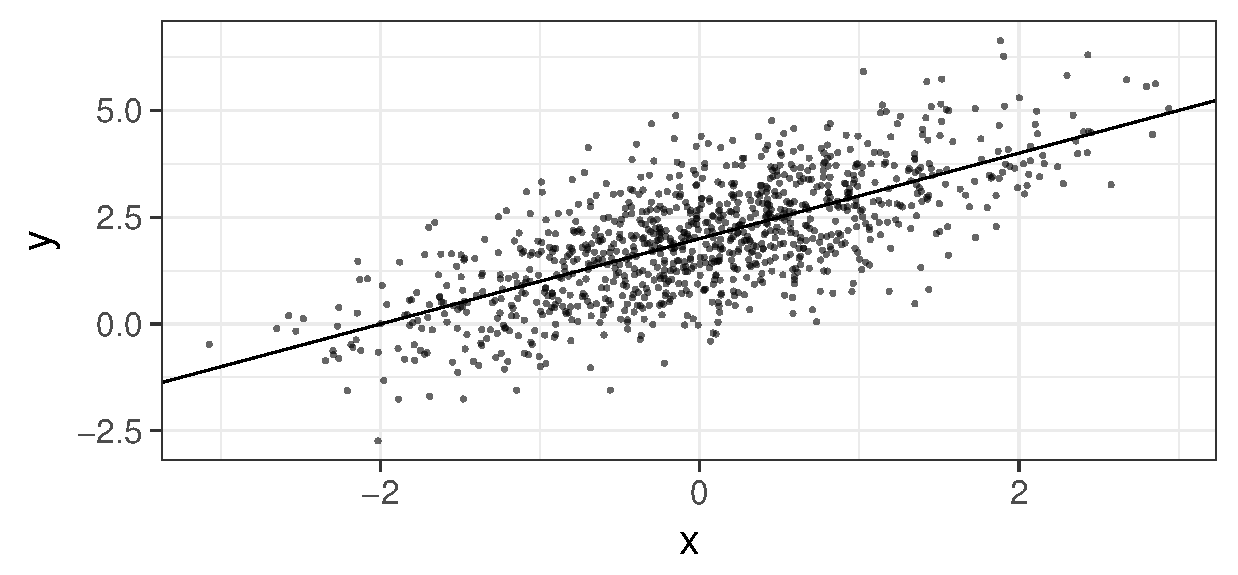
\includegraphics[width=\textwidth]{lin_reg_example_1.pdf}
  \caption{Datos generados para una regresión lineal simple.}
  \label{fig:reg_lineal_ejemplo}
\end{figure}

\begin{figure}[H]
  \centering
  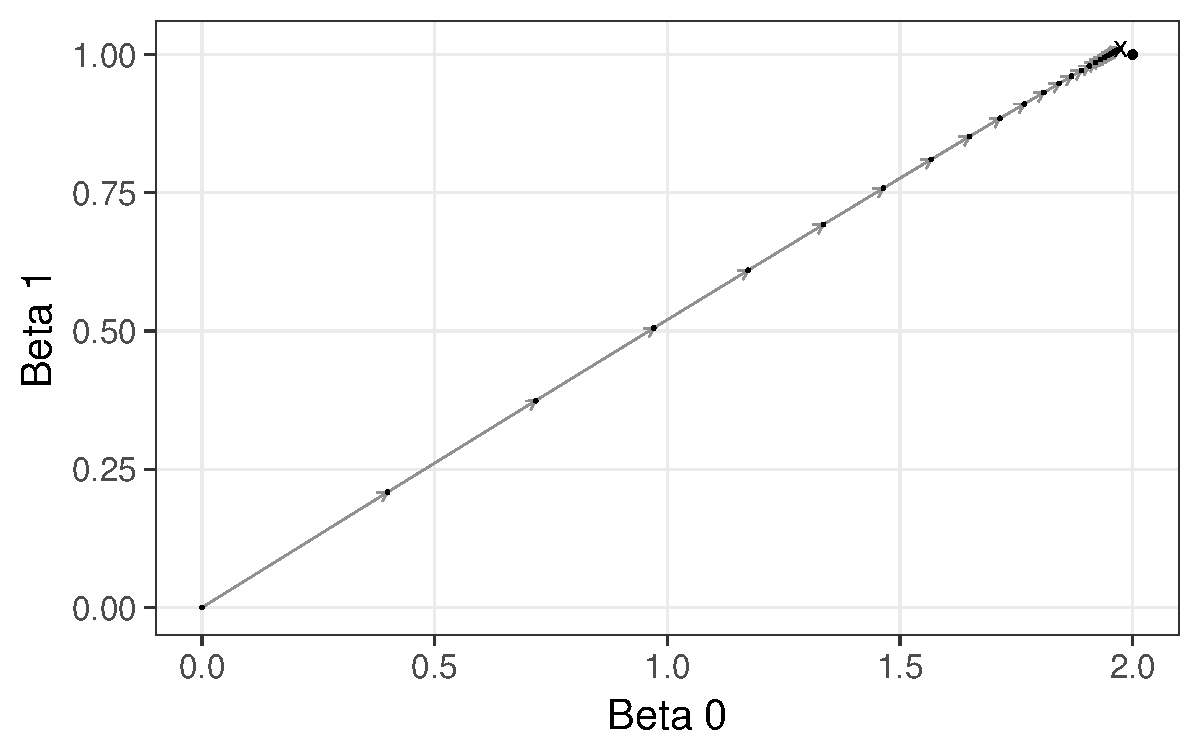
\includegraphics[width=\textwidth]{lin_reg_example_1_GD_iter.pdf}
  \caption{Iteraciones del algoritmo de descenso en gradiente para regresión lineal.}
  \label{fig:reg_lineal_ejemplo_GD_iter}
\end{figure}

%%%%%%%%%%%%%%%%
%%% Reg logística
%%%%%%%%%%%%%%%%

En el caso de regresión logística, en el caso general, se busca minimizar la función de pérdida llamada \textbf{devianza}, definida como

\begin{equation}
  \label{eq:devianza_reg_log}
  L(x, \beta) = - \frac{2}{n} \sum_{i=1}^{n} \left[ y_i \log(h(\beta^T x_i)) + (1-y_i) \log(1-h(\beta^T x_i)) \right] = 
     - \frac{2}{n} \sum_{i=1}^{n}{\ell_i(\beta)}
\end{equation}

donde 
$$
  \beta^T x_i = \sum_{j=0}^{p}{\beta_j x_{ij}},
$$ 

$$
  h(w) = \frac{e^w}{1+e^w}
$$ 

y 

$$
\ell_i(x) = y_i \log(h(\beta^T x_i)) + (1-y_i) \log(1-h(\beta^T x_i)).
$$

Se tiene que 

$$
  \frac{\partial L}{\partial \beta_j} = -\frac{2}{n} \sum_{i = 1}^n { \frac{\partial \ell_i}{\partial \beta_j} }
$$

y además, usando el hecho de que $h'(w) = h(w)(1-h(w))$, se tiene

\begin{equation}
  \label{eq:derivacion_ell_i_reg_log}
  \begin{split}
    \frac{\partial \ell_i}{\partial \beta_j} & = 
      \frac{y_i h'(\beta^T x_i) x_{ij} }  {h(\beta^T x_i)} + \frac{(1 - y_i) (-1) h'(\beta^T x_i) x_{ij}} {1 - h(\beta^T x_i)} \\
      & = \frac{h'(\beta^T x_i) x_{ij} y_i}{h(\beta^T x_i)} - \frac{(1 - y_i) h'(\beta^T x_i) x_{ij}}{1 - h((\beta^T x_i))} \\
      & = h'(\beta^T x_i) x_{ij} \left(\frac{y_i}{h(\beta^T x_i)} - \frac{1-y_i}{1-h(\beta^T x_i)} \right) \\
      & = h'(\beta^T x_i) x_{ij} \left(\frac{y_i - y_i h(\beta^T x_i) - 
          h(\beta^T x_i) + y_i h(\beta^T x_i)}{h(\beta^T x_i)(1-h(\beta^T x_i))} \right) \\
      & = x_{ij}(y_i - h(\beta^T x_i)).
  \end{split}
\end{equation}

Por lo tanto, se tiene que 

$$
  \frac{\partial L}{\partial \beta_j} = -\frac{2}{n} \sum_{i = 1}^n { x_{ij}(y_i - h(\sum_{j=0}^{p}{\beta_j x_{ij}})) },
$$

donde nuevamente $x_{i1} = 1$ para toda $i \in \left\{1, \hdots, n \right\}$.


En el ejemplo implementado, se generó un vector $x \in \mathbb{R}^n$ con $n = 1000$ tal que $x_i \sim N(0, 1)$ para cada $i \in \left\{1, \hdots, n \right\}$ y se construyó la variable auxiliar $p_i = \frac{1}{\exp \left( - \beta_0 - \beta_1 x_i \right)}$ con $\beta_0 = 1$ y $\beta_1 = 4$. Finalmente, la variable respuesta $y$ se construyó simulando una variables aleatorias Bernoulli, de tal forma que $y_i \sim Bern(p_i)$. Los datos generados se pueden ver en la figura \ref{fig:reg_log_ejemplo}.

Entonces, para minimizar la devianza \ref{eq:devianza_reg_log}, exactamente igual que en el otro caso, se empieza con un vector $\beta^0 \in \mathbb{R}^2$, y en cada iteración, se actualiza 

$$
  \beta^{k+1} = \beta^k - \alpha_k \nabla_{\beta} L(x, \beta)
$$

hasta un criterio de paro. En este caso, el criterio de paro fue un poco más estricto: la norma del gradiente $\nabla_{\beta} L(x, \beta)$ debía ser menor a $0.0001$, o el cociente de normas entre cada iteración fuera mayor a $0.8$, o que se excediera de 500 iteraciones. El vector de parámetros inicial fue $\beta^0 = (-10, 10)^T$. En este caso se hizo \textit{backtracking} con un valor inicial $\alpha_0 = 3$.

Los valores del vector de parámetros en cada iteración se pueden ver en la figura \ref{fig:reg_log_ejemplo_GD_iter}. El punto grande que se ve en la figura es el valor real de los parámetros (i.e. 1 y 4), y el tache que se ve es el valor obtenido utilizando el paquete \texttt{glm} de \texttt{R}. Se puede ver que el algoritmo implementado converge a estos valores y, nuevamente, el valor obtenido con el método implementado es exactamente igual al que regresa el paquete utilizado (\texttt{glm}).


\begin{figure}[H]
  \centering
  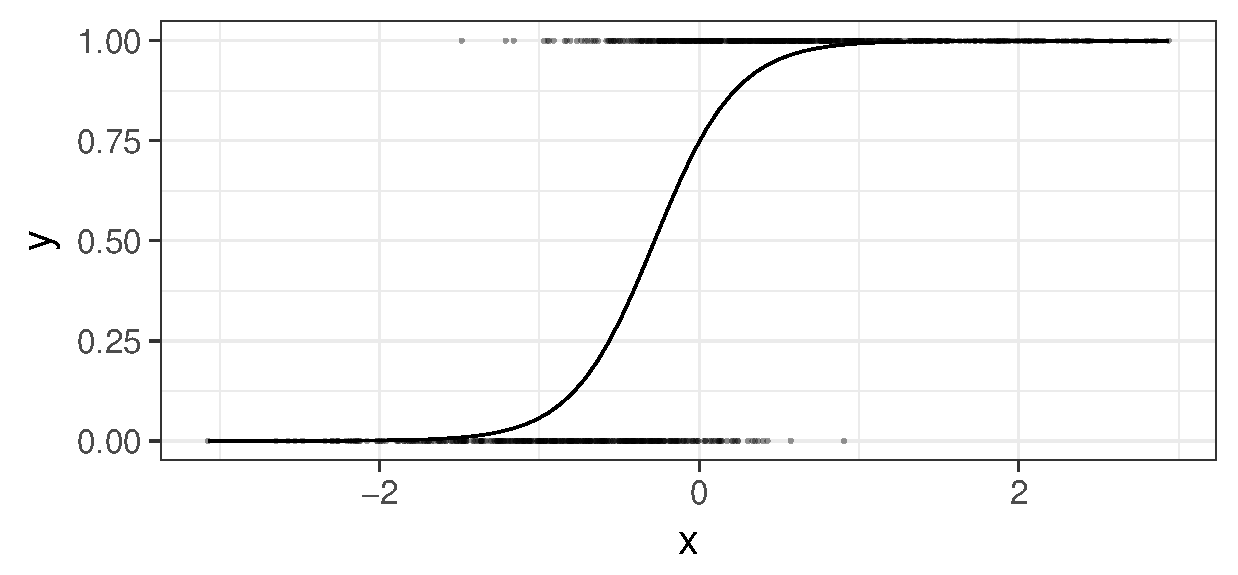
\includegraphics[width=0.9\textwidth]{log_reg_example_1.pdf}
  \caption{Datos generados para una regresión logística.}
  \label{fig:reg_log_ejemplo}
\end{figure}


\begin{figure}[H]
  \centering
  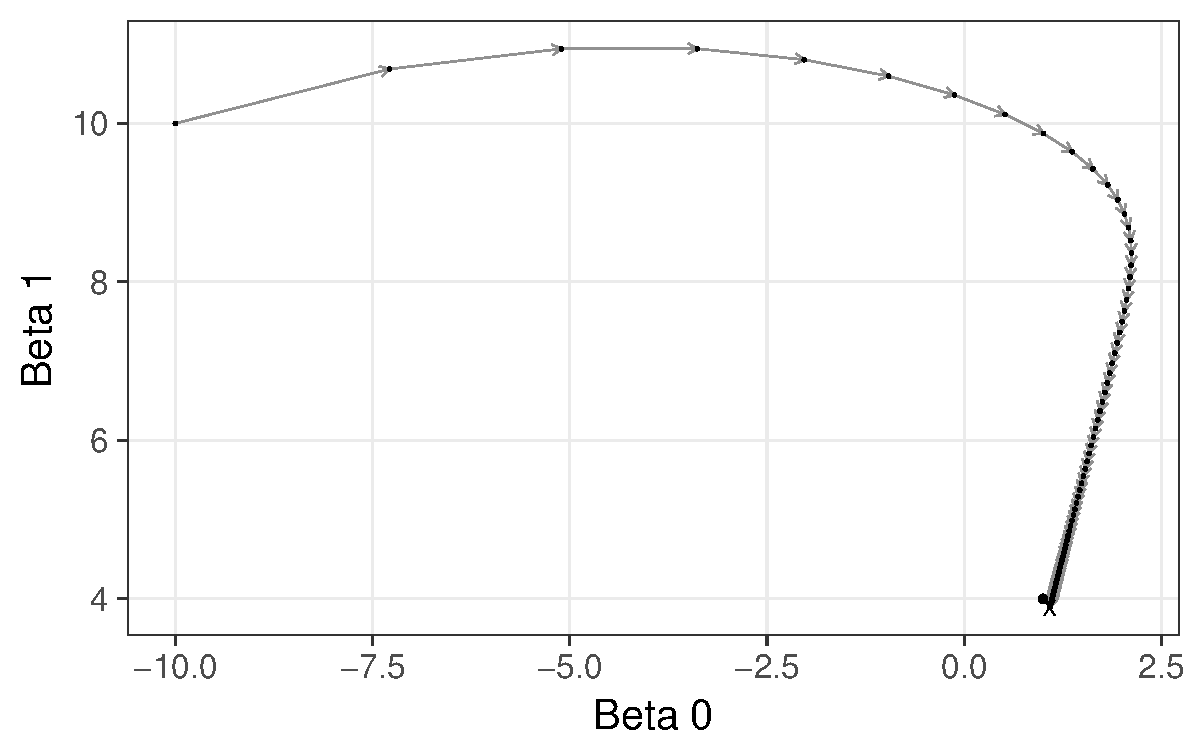
\includegraphics[width=0.9\textwidth]{log_reg_example_1_GD_iter.pdf}
  \caption{Iteraciones del algoritmo de descenso en gradiente para regresión logística.}
  \label{fig:reg_log_ejemplo_GD_iter}
\end{figure}





%%%%%%%%%%%%%%%%%%%%%%%%%%%%%%%%%%%%%%%%%%%%%%%%%%%%%%
%%% SGD
%%%%%%%%%%%%%%%%%%%%%%%%%%%%%%%%%%%%%%%%%%%%%%%%%%%%%%

\subsection{Descenso en gradiente estocástico}
\label{sec:descenso_gradiente_estocastico}

En el aprendizaje estadístico es muy común encontrar problemas de optimización de la forma

\begin{equation}
  \label{eq:perd_gral_apr_est}
  \min_{\theta \in \mathbb{R}^p} L(x, \theta), \quad \text{donde} \, \, 
    L(\theta) = \frac{1}{n} \sum_{i = 1}^n { \psi_i(x, \theta) }.
\end{equation}

En los ejemplos de la subsección \ref{sec:descenso_gradiente} se puede ver esto con claridad: las funciones de pérdida a minimizar son de la forma \ref{eq:perd_gral_apr_est}. El método de descenso en gradiente presentado en \ref{sec:descenso_gradiente} utiliza iteraciones de la forma de la ecuación \ref{eq:iteracion_descenso_grad}, es decir, 

\[
  \theta_{k+1} = \theta_k - \alpha_k \nabla L(\theta_k) :=\theta_k - \frac{\alpha_k}{n} \sum_{i = 1}^n \nabla \psi_i(\theta_k),
\]

lo cual involucra la evaluación de $n$ gradientes para después promediarlos. En los casos de aprendizaje automático de gran escala, el número de observaciones $n$ es grande, por lo que calcular estos gradientes puede resultar costoso. Debido a esto, surgen los métodos como descenso en gradiente estocástico, en los cuales el número de gradientes a evaluar no depende de $n$, sino que es constante. Este método utiliza iteraciones de la forma

\[
  \theta_{k+1} = \theta_k - \frac{\alpha_k}{n} \nabla \psi_{i_k}(\theta_k),
\]

donde $i_k \in \left\{1, 2, \hdots, n \right\}$ es escogido aleatoriamente. El gradiente $\nabla \psi_{i_k}(\theta_k)$ es un estimador insesgado de $\nabla L(\theta_k)$. De esta forma, cada iteración es muy barata pues involucra la evaluación de solamente un gradiente. Puede suceder que alguna $\nabla \psi_{i_k}(\theta_k)$ particular no otorgue una dirección de descenso partiendo de $\theta_k$, pero, intuitivamente, en promedio sí se dan direcciones de descenso, de tal forma que le sucesión $\left\{ \theta_0, \theta_1, \hdots \right\}$ puede ser guiada a un minimizador $\theta^*$.

Para ilustrar este método, se implementaron los dos mismos ejemplos que en la sección \ref{sec:descenso_gradiente}, es decir, la regresión lineal y la regresión logística.


%%%%%%%%%%%%%%%%
%%% Reg lineal
%%%%%%%%%%%%%%%%

En el caso de la regresión lineal, se desea minimizar la pérdida cuadrática definida en la ecuación \ref{eq:perd_cuadratica_reg_lineal}. Aquí, si se utiliza la notación utilizada en la ecuación \ref{eq:perd_gral_apr_est}, cada $\psi_i(x, \theta)$ es 

$$
  \psi_i(x, \theta) = \left( y_i - \beta_0 - \beta_1 x_{i1} - \hdots  \beta_p x_{ip} \right)^2 = \ell_i^2(x, \beta),
$$ 

con $\ell_i(x, \beta)$ definido en la ecuación \ref{eq:ele_i_reg_lineal}. Se puede ver que la derivada parcial de $\psi_i(x, \beta)$ respecto a cada $\beta_j$ con $j \in \left\{ 0, \hdots, p \right\}$ es

\[
  \frac{\partial \psi_i}{\partial \beta_j} = \frac{\partial \ell^2_i}{\partial \beta_j} = -2 x_{ij} \ell_i(x, \beta),
\]

por lo que la dirección de avance en cada iteración del algoritmo es

\[
  \nabla_{\beta} \psi_i(x, \beta) = 
    \left( \frac{\partial \psi_i}{\partial \beta_0}, \hdots, \frac{\partial \psi_i}{\partial \beta_p} \right).
\]

Nuevamente, el vector de parámetros iniciales fue $\beta^0 = (0, 0)^T$.  El criterio de paro era que la norma del gradiente $\nabla_{\beta} L(x, \beta)$ fuera menor a $0.000001$, que se excediera de 300 iteraciones o que la norma dos al cuadrado de las diferencias del vector de parámetros entre una iteración y otra (i.e. $\norm{\beta^{k+1} - \beta^k}^2_2$) fuera menor a $10^{-15}$. 

Los valores del vector de parámetros en cada iteración se pueden ver en las figuras \ref{fig:lin_reg_example_1_SGD_iter_all} y \ref{fig:lin_reg_example_1_SGD_each_epoch}. Para entender mejor estas imágenes, es pertinente explicar qué es un \textit{epoch}. Un \textit{epoch} es un conjunto de $n$ accesos al conjunto de datos. Es decir, en cada \textit{epoch}, se evalúan los gradientes de todos los datos en el conjunto de entrenamiento.

En la figura \ref{fig:lin_reg_example_1_SGD_iter_all} se muestran los valores de los parámetros para todos los gradientes en todos los \textit{epochs}. En la figura \ref{fig:lin_reg_example_1_SGD_each_epoch} se muestran solo los valores al final de cada \textit{epoch} para tener mayor claridad en la visualización. Se puede apreciar en la figura \ref{fig:lin_reg_example_1_SGD_iter_all} que, a diferencia de la figura \ref{fig:reg_lineal_ejemplo_GD_iter} donde las direcciones de descenso se ven más uniformes hacia una misma dirección, las direcciones van hacia todos lados en una especie de \textit{zig-zag} que eventualmente llega a la solución.

En ambas figuras se muestra un punto grande que representa el valor real de los parámetros ($\beta_0=2$ y $\beta_1 = 1$) y el tache que representa el valor obtenido utilizando el paquete \texttt{lm} de \texttt{R}, pero en la figura \ref{fig:lin_reg_example_1_SGD_iter_all} no se alcanza a distinguir tan bien, pero en ambas imágenes se puede ver que el algoritmo implementado converge a los valores deseados.

\begin{figure}[H]
  \centering
  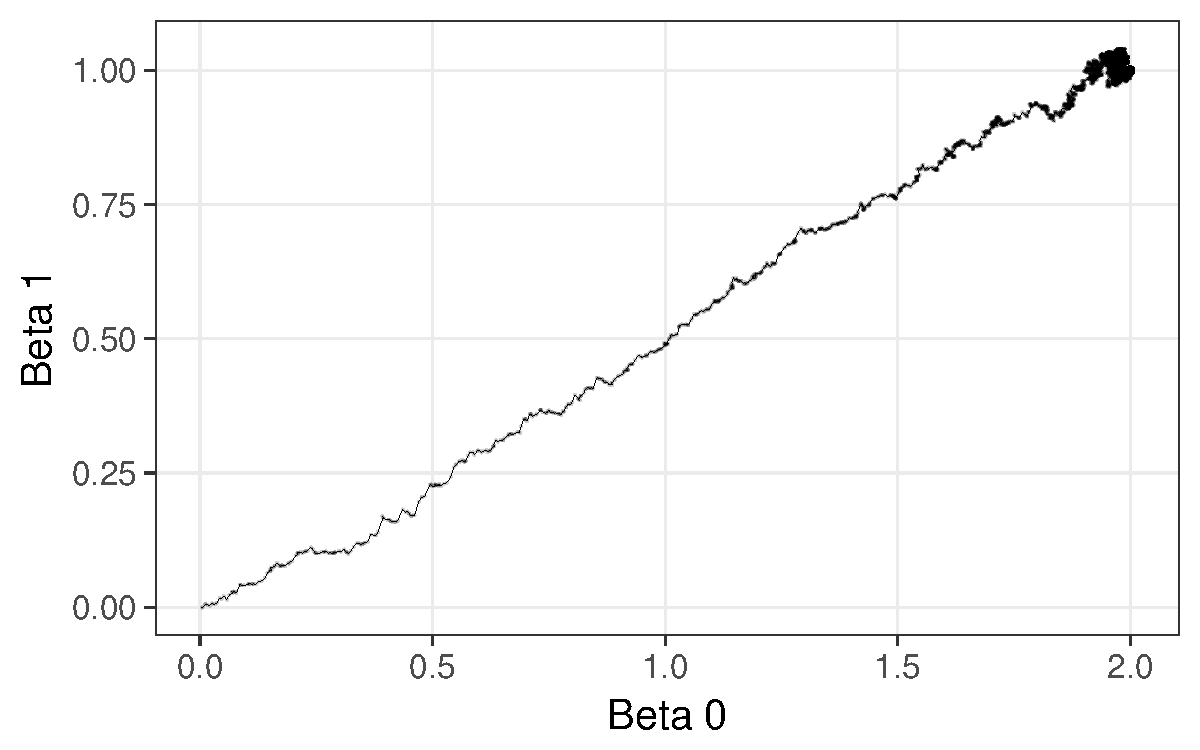
\includegraphics[width=0.9\textwidth]{lin_reg_example_1_SGD_iter_all.pdf}
  \caption{Iteraciones del algoritmo de descenso en gradiente estocástico para regresión lineal.}
  \label{fig:lin_reg_example_1_SGD_iter_all}
\end{figure}

\begin{figure}[H]
  \centering
  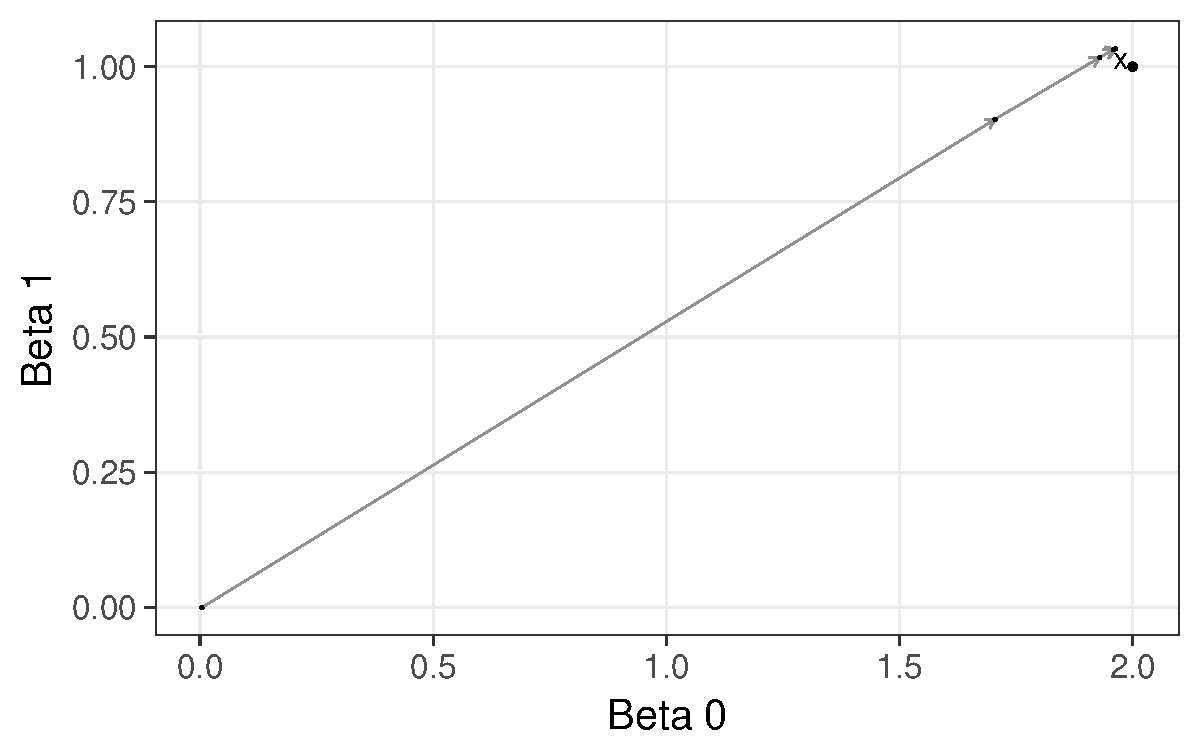
\includegraphics[width=0.9\textwidth]{lin_reg_example_1_SGD_each_epoch.pdf}
  \caption{Iteraciones del algoritmo de descenso en gradiente para regresión lineal. Cada flecha apunta al valor de los parámetros después de cada \textit{epoch}.}
  \label{fig:lin_reg_example_1_SGD_each_epoch}
\end{figure}



%%%%%%%%%%%%%%%%
%%% Reg logística
%%%%%%%%%%%%%%%%

Para la regresión logística ya se tienen hechos casi todos los cálculos necesarios en la subsección \ref{sec:descenso_gradiente}. Con la notación utilizada en la ecuación \ref{eq:perd_gral_apr_est}, cada $\psi_i(x, \theta)$ es 

$$
  \psi_i(x, \theta) = y_i \log(h(\beta^T x_i)) + (1-y_i) \log(1-h(\beta^T x_i)) = \ell_i(x, \beta).
$$ 

Además, en las ecuaciones \ref{eq:derivacion_ell_i_reg_log} se llega a que

\[
  \frac{\partial \ell_i}{\partial \beta_j} = \frac{\partial \psi_i}{\partial \beta_j} = x_{ij}(y_i - h(\beta^T x_i)).
\]

Por lo que ya se tiene todo lo necesario. En la implementación, el criterio de paro fue el mismo que en descenso en gradiente estocástico para regresión lineal: que la norma del gradiente $\nabla_{\beta} L(x, \beta)$ fuera menor a $0.000001$, que se excediera de 300 iteraciones o que la norma dos al cuadrado de las diferencias del vector de parámetros entre una iteración y otra fuera menor a $10^{-15}$. 

Los valores del vector de parámetros en cada iteración se pueden ver en las figuras \ref{fig:log_reg_example_1_SGD_iter_all} y \ref{fig:log_reg_example_1_SGD_each_epoch}. Las explicaciones de estas dos imágenes son análogas a las de regresión lineal. Nuevamente, el valor obtenido con el método implementado converge al valor real y al que se obtuvo con el paquete \texttt{glm}.

\begin{figure}[H]
  \centering
  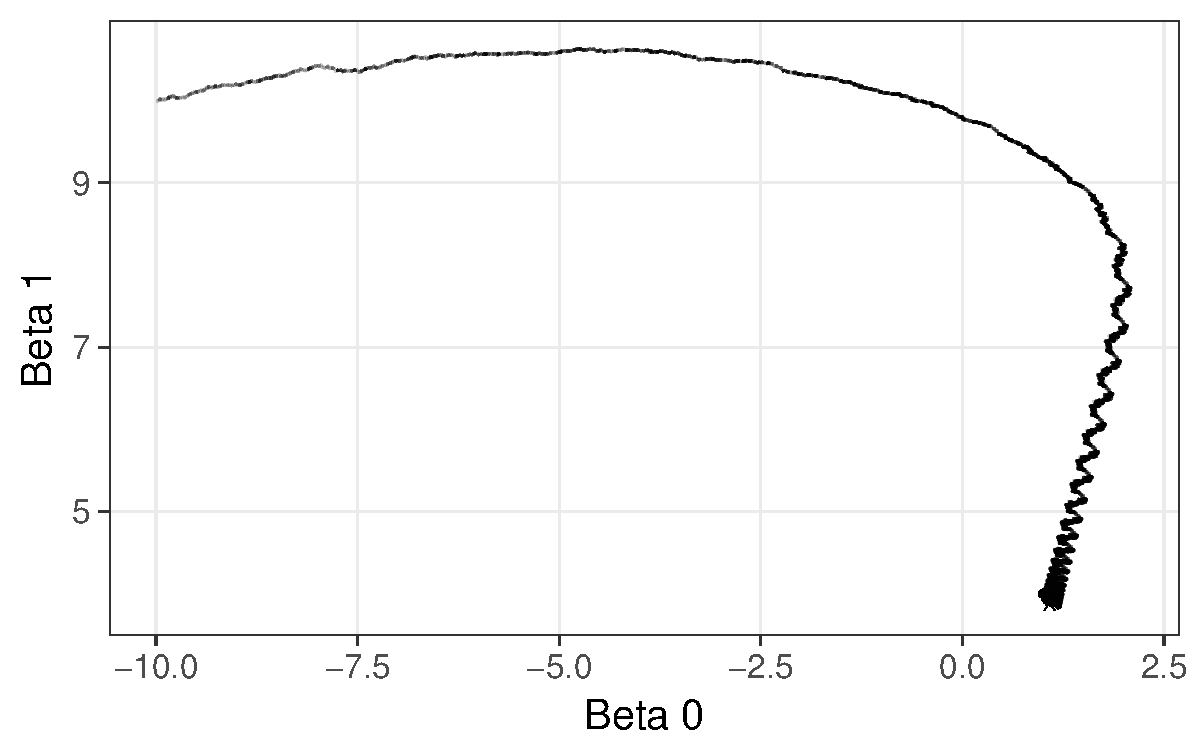
\includegraphics[width=0.9\textwidth]{log_reg_example_1_SGD_iter_all.pdf}
  \caption{Iteraciones del algoritmo de descenso en gradiente para regresión logística.}
  \label{fig:log_reg_example_1_SGD_iter_all}
\end{figure}


\begin{figure}[H]
  \centering
  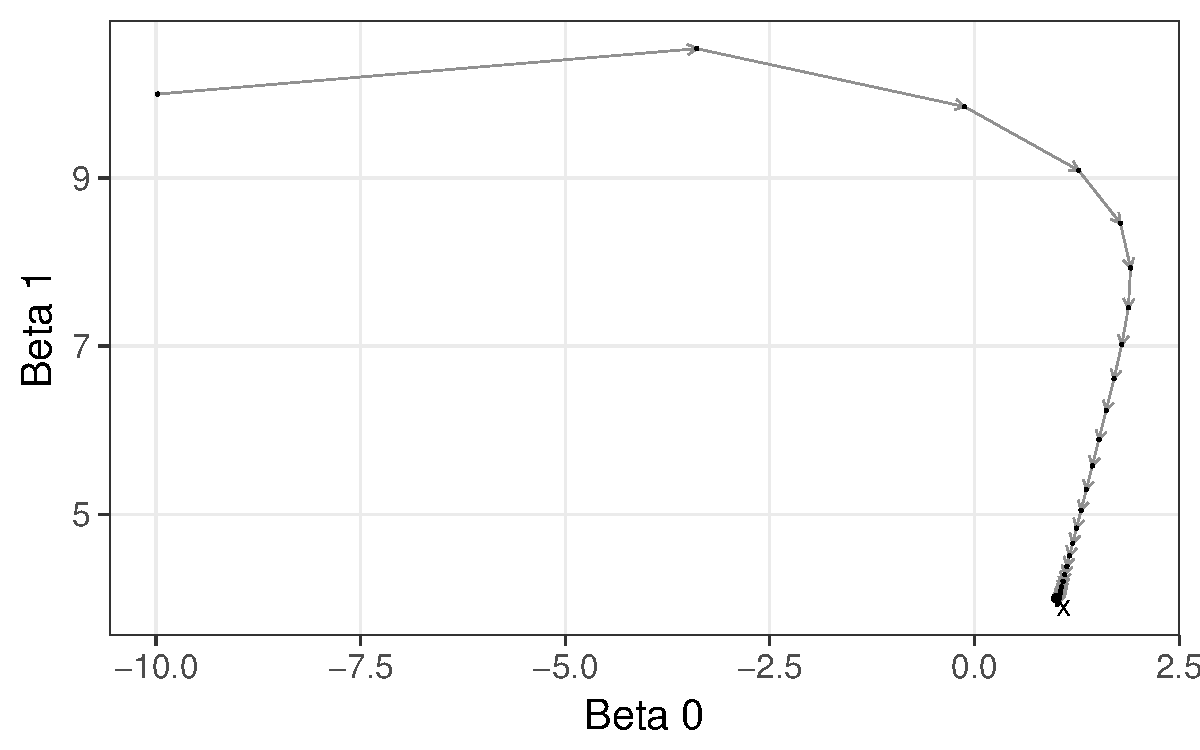
\includegraphics[width=0.9\textwidth]{log_reg_example_1_SGD_each_epoch.pdf}
  \caption{Iteraciones del algoritmo de descenso en gradiente para regresión logística. Cada flecha apunta al valor de los parámetros después de cada \textit{epoch}.}
  \label{fig:log_reg_example_1_SGD_each_epoch}
\end{figure}




%%%%%%%%%%%%%%%%%%%%%%%%%%%%%%%%%%%%%%%%%%%%%%%%%%%%%%
%%%%%%%%%%%%%%%%%%%%%%%%%%%%%%%%%%%%%%%%%%%%%%%%%%%%%%
%%%%%%%%%%%%%%%%%%%%%%%%%%%%%%%%%%%%%%%%%%%%%%%%%%%%%%
%%% Sistemas de recomendación
%%%%%%%%%%%%%%%%%%%%%%%%%%%%%%%%%%%%%%%%%%%%%%%%%%%%%%
%%%%%%%%%%%%%%%%%%%%%%%%%%%%%%%%%%%%%%%%%%%%%%%%%%%%%%
%%%%%%%%%%%%%%%%%%%%%%%%%%%%%%%%%%%%%%%%%%%%%%%%%%%%%%

\section{Sistemas de recomendación}

Las definiciones de esta sección fueron obtenidas de \cite{recommenderlab_manual}, \cite{koren2009matrix} y \cite{leskovec_mining_2014}.

El objetivo de los sistemas de recomendación es predecir las respuestas de los usuarios a distintas opciones. Dos clasificaciones muy amplias de los sistemas de recomendación son: basados en contenido y filtrado colaborativo. Existen dos grandes tipos de sistemas de recomendación de acuerdo a las técnicas que usan.

\begin{itemize}
\item Basados en contenido: A partir de características y propiedades de los productos (por ejemplo, género, actores, país de origen, año, etc.) intentamos predecir el gusto por el producto construyendo variables derivadas del contenido de los artículos (como qué actores salen, año, etc.).
\item Colaborativos: A partir de usuarios y productos se construyen medidas de similitud en el sentido de que les han gustado los mismos productos o que les gustaron a las mismas personas. Así, los productos recomendados a un usuario son los que le gustaron a otros usuarios.
\end{itemize}

En este trabajo se supone que se tiene una matriz de calificaciones $R$, tal que las filas representan usuarios que calificaron a los productos representados en las columnas de la siguiente forma:

\begin{center}
\begin{tabular}{ c | c  c c c c}
    & $P_1$ & $P_2$ & $P_3$ & $\cdots$ & $P_n$ \\
  \hline                       
  $U_1$ &   1 &     2 &     3 & $\cdots$ &      - \\
  $U_2$ &   4 &     - &     4 & $\cdots$  &     -\\
  $\vdots$ & $\vdots$ & $\vdots$ & $\vdots$ & $\ddots$ & $\vdots$\\
  $U_m$ &   - &     - &     1 & $\cdots$ &      3\\
  \hline  
\end{tabular}
\end{center}

donde cada $P_i$ es el producto i-ésimo que se ofrece y $U_i$ es el usuario i-ésimo que ha calificado el producto correspondiente. Los espacios donde hay guiones representan datos faltantes. Es usual que este tipo de matrices tengan la mayor parte de las entradas faltantes, pues no todos los usuarios han visto todas las películas, o calificado todos los productos. El objetivo del sistema de recomendación es llenar los espacios faltantes mediante una predicción y recomendar los productos que tienen una predicción alta. Notar que aquí se considera que ya se tiene la matriz de calificaciones, lo cual a veces, en la práctica, puede ser un trabajo difícil y haya que pedir a usuarios que califiquen productos.

\subsection{Basados en contenido}

Para este tipo de recomendaciones se construye un \textbf{perfil} para cada producto. Como se había mencionado, este perfil puede contener el género, los actores, país de origen, etc. Esto puede ser más sencillo en el caso de películas pues existen fuentes de información sobre las películas como \textit{Internet Movie Database (IMDb)}; pero con documentos o imágenes, por ejemplo, no siempre se tiene esta información, así que es necesario la construcción de variables a través de \textit{tags}, palabras clave y, en el caso de texto, tal vez un modelo de lenguaje.

Una vez construidos los perfiles, el proceso que queda es de alguna forma emparejar los gustos del usuario obtenidos de la matriz de utilidad con los perfiles de los productos.

Un ejemplo muy sencillo es el siguiente. Supóngase dos películas con 8 actores en total ($A_1$, ..., $A_8$), cinco actores cada una y que dos actores están en las dos películas, y que además las calificaciones promedio de cada película son 3 y 4. Entonces los perfiles de dos películas se ven como:

\begin{center}
  \begin{tabular}{ c | c  c c c c c c c c}
      & $A_1$ & $A_2$ & $A_3$ & $A_4$ & $A_5$ & $A_6$ & $A_7$ & $A_8$ & Calif \\
      \hline                       
      $P_1$ & 0 & 1 & 1 & 0 & 1 & 1 & 0 & 1 & 3 \\
      $P_2$ & 1 & 1 & 0 & 1 & 0 & 1 & 1 & 0 & 4 \\
      \hline  
  \end{tabular}
\end{center}

Con esta información se puede obtener una medida de similitud entre las películas. Una medida muy utilizada es la similitud coseno, definida como

\[
  sim(P_1, P_2) = \frac{P_1^T P_2}{\norm{P_1} \norm{P_2} }.
\]

Supóngase ahora que los usuarios $U_k$ y $U_j$ solo han calificado dos películas. Si el usuario $U_k$ calificó con 2 y 4 las películas $P_1$ y $P_2$ respectivamente y si el usuario $U_j$ calificó con 4 y 4 las películas $P_1$ y $P_2$ respectivamente, entonces se puede ver esto en forma matricial:

\begin{center}
  \begin{tabular}{ c | c  c }
      & $P_1$ & $P_2$ \\
    \hline                       
    $U_k$ & 2 & 4 \\
    $U_j$ & 4 & 4 \\
    \hline  
  \end{tabular}
\end{center}

Tiene sentido centrar las calificaciones por usuario (restarle la media) para reducir un poco la heterogeneidad de la escala. Con heterogeneidad de la escala, uno se refiere a que algunos usuarios tienden a calificar más estricto que otros; entonces se tiene:

\begin{center}
\begin{tabular}{ c | c  c }
    & $P_1$ & $P_2$ \\
  \hline                       
$U_k$ & -1 & 1 \\
$U_j$ & 0 & 0 \\
  \hline  
\end{tabular}
\end{center}

Así, para el usuario $U_k$ se tiene que los perfiles para cada película se ven como:

\begin{center}
\begin{tabular}{ c | c  c c c c c c c c}
    & $A_1$ & $A_2$ & $A_3$ & $A_4$ & $A_5$ & $A_6$ & $A_7$ & $A_8$ & Calif \\
  \hline                       
$P_1$ & 0 & -1 & -1 & 0 & -1 & -1 & 0 & -1 & 2 \\
$P_2$ & 1 & 1 & 0 & 1 & 0 & 1 & 1 & 0 & 4 \\
  \hline  
\end{tabular}
\end{center}

Y para el usuario $U_j$ se ven como:

\begin{center}
\begin{tabular}{ c | c  c c c c c c c c}
    & $A_1$ & $A_2$ & $A_3$ & $A_4$ & $A_5$ & $A_6$ & $A_7$ & $A_8$ & Calif \\
  \hline                       
$P_1$ & 0 & 4 & 4 & 0 & 4 & 4 & 0 & 4 & 4 \\
$P_2$ & 4 & 4 & 0 & 4 & 0 & 4 & 4 & 0 & 4 \\
  \hline  
\end{tabular}
\end{center}

Entonces, para el perfil general de cada usuario, se promedian por película los perfiles de cada uno y se obtiene

\begin{center}
\begin{tabular}{ c | c  c c c c c c c c}
    & $A_1$ & $A_2$ & $A_3$ & $A_4$ & $A_5$ & $A_6$ & $A_7$ & $A_8$ & Calif \\
  \hline                       
$U_k$ & 0.5 & 0 & -0.5 & 0.5 & -0.5 & 0 & 0.5 & -0.5 & 3 \\
$U_j$ & 2 & 4 & 2 & 2 & 2 & 4 & 2 & 2 & 4 \\
  \hline  
\end{tabular}
\end{center}

Con esto se puede estimar qué tanto le va a gustar a un usuario una película calculando la similitud coseno entre el perfil del usuario y el perfil de la película. Esta forma es muy rudimentaria y sencilla, pero puede servir como base para otros modelos.

\subsection{Colaborativos}

\subsubsection{Modelo base} \label{sec:modelo_base}

En esta sección se construye un modelo base muy sencillo para hacer predicciones, y el cual sirve como comparación con otros modelos más complejos. Para este modelo se supone que los artículos y los usuarios tienen sesgos, o sea, hay usuarios que tienden a calificar más alto, o a ser más estrictos y calificar más bajo; al mismo tiempo, puede haber artículos que tiendan a recibir calificaciones más altas; y que gran parte de la calificación observada se debe a efectos asociados a estos sesgos.

Sea $\mu$ la media general de todos los artículos y todos los usuarios, entonces la predicción del modelo base es

\[
\hat{r_{ij}} = \mu + a_i + b_j
\]

donde $a_i$ es la desviación del usuario $i$ respecto a la media general y $b_j$ es la desviación del artículo $j$ respecto a la media general.

Una forma de estimar los sesgos es calculando

\[
a_i = \frac{1}{M_i} \sum_t r_{it} - \mu,
\]

y 

\[
b_j = \frac{1}{N_j} \sum_s r_{sj} - \mu,
\]

donde donde $M_i$ es el número de artículos calificados por el usuario $i$ y $N_j$ es el número de calificaciones que tiene el artículo $j$.

Otra forma un poco más precisa es resolver el problema de mínimos cuadrados regularizado

\[
\min_{b} \sum_{(i, j) \in A} \left( r_{ij} - \mu - a_i - b_j \right) ^2 + \lambda \left( \sum_{i} a_i^2 + \sum_{j} b_j^2 \right)
\]

donde $r_{ij}$ es la calificación del usuario $i$ del artículo $j$, $A$ es el conjunto de usuarios y artículos para los cuales se conoce la calificación $r_{ij}$, $ \vert A \vert$ es la cardinalidad de $A$ (o sea, el total de artículos calificados por todos los usuarios) y $\lambda$ es un término de regularización que evita el sobreajuste.

A este sencillo modelo se le pueden agregar otros términos de regularización que ayuden a disminuir el ruido causado por artículos y usuarios con pocas calificaciones, al encoger las calificaciones a la media. Una vez que se calcularon $a_i$ y $b_j$ usando cualquiera de los métodos mencionados, se hace la predicción

\begin{equation}
  \label{ec:modelo_base}
  r_{ij} = \mu + \frac{M_i}{\gamma + M_i} a_i + \frac{N_j}{\gamma + N_j}b_j
\end{equation}

donde $M_i$ es el número de artículos que ha calificado el usuario $i$, $N_j$ es el número de calificaciones que tiene el artículo $j$, y $\gamma$ es el parámetro de regularización.

\subsubsection{Métodos de vecindario}

Este tipo de modelos se centran en la similitud de los usuarios y los artículos. Los usuarios son similares si los vectores que los representan (es decir, las filas en la matriz de calificaciones) están cercanos de acuerdo a alguna similitud definida. Una recomendación para un usuario $i$ se hace al ver a los usuarios más parecidos a $i$ y recomendando artículos que hayan sido del agrado de estos usuarios parecidos.

El primer problema con estos métodos surge al definir una medida de similitud entre artículos o usuarios. Dos medidas muy utilizadas son la similitud de Jaccard y, nuevamente, la similitud coseno. La similitud de Jaccard de dos vectores $A$ y $B$ está definida como el cociente de la cardinalidad de la intersección y la cardinalidad de la unión de los dos vectores:

\[
  J(A, B) = \frac{\vert A \cap B \vert}{\vert A \cup B \vert}.
\]

En el caso de una matriz de calificaciones binaria, la similitud Jaccard tendría más sentido, pero si son calificaciones explícitas conviene más utilizar similitud coseno. Una desventaja de utilizar la similitud coseno es que los elementos faltantes son tratados como $0$, lo cual tiene el efecto de tratar la falta de calificación como disgusto hacia el artículo. Una forma de solucionar esto es centrando las calificaciones por usuario al restar la media, de esta forma el faltante al ser tratado como cero tiene el efecto de que al usuario ni le gusta ni le disgusta el artículo.

Una forma de hacer predicciones de calificaciones para un usuario $i$ y un artículo $j$ es encontrar un vecindario de los $n$ usuarios más parecidos a $i$ y tomar el promedio de las calificaciones del artículo $j$. O de forma dual, se podría encontrar un vecindario con los $n$ artículos más parecidos a $j$ y tomar el promedio de las calificaciones que el usuario $i$ ha dado a esos artículos. Aquí se hace una vertiente en los métodos de vecindario, dependiendo de si se centran en las similitudes de los usuarios o de los artículos.

\paragraph{Basados en usuarios}

Este tipo de algoritmos pretenden imitar las recomendaciones de boca en boca al asumir que los usuarios con preferencias similares calificarán los artículos de forma similar. De esta manera, para hacer una predicción para el usuario $i$ y el artículo $j$ habría que encontrar un vecindario de $i$, denotado como $N(i)$, y tomar el promedio de las calificaciones en el vecindario:

\begin{equation}\label{eq:predic_modelo_usuario_sencillo}
 \hat{r_{ij}} = \frac{\sum_{a \in N(i)} r_{aj}}{\vert N(i) \vert}.
\end{equation}

La ecuación \ref{eq:predic_modelo_usuario_sencillo} está ignorando el hecho de que algunos usuarios en el vecindario son más similares a otros, por lo que es una buena idea tener un ponderador de similitud. Así, en lugar de \ref{eq:predic_modelo_usuario_sencillo}, la predicción es

\begin{equation}\label{eq:predic_modelo_usuario_ponderado}
 \hat{r_{ij}} = \frac{\sum_{a \in N(i)} s_{ia} r_{aj}}{\sum_{a \in N(i)} s_{ia}},
\end{equation}

donde $s_{ia}$ es la similitud entre el usuario $i$ y el usuario $a$ perteneciente al vecindario de $i$.

\paragraph{Basados en artículos}

Este tipo de algoritmos asumen que los usuarios prefieren artículos que son similares a otros artículos que les gustaron. Muchas veces este tipo de sistemas producen información más confiable porque es más sencillo encontrar artículos del mismo género que encontrar usuarios a los que solo les gustan artículos de un solo género. En este caso, para hacer una predicción para el usuario $i$ y el artículo $j$ habría que encontrar un vecindario de $j$, denotado como $N(j)$, y tomar el promedio (ponderado por nivel de similitud para mejor estimación) de las calificaciones que el usuario ha hecho a los artículos en $N(j)$, es decir

\begin{equation}\label{predic_modelo_articulo_ponderado}
 \hat{r_{ij}} = \frac{\sum_{a \in N(j)} s_{ja} r_{ia}}{\sum_{a \in N(j)} s_{ja}},
\end{equation}

donde $s_{ja}$ es la similitud entre el artículo $j$ y el artículo $a$ perteneciente al vecindario de $j$.


\subsubsection{Métodos de factorización de matrices} \label{sec:modelo_factorizacion}

\paragraph{Modelo básico de factorización de matrices}

La idea de la factorización de matrices proviene de los modelos de factores latentes, en los cuales se supone que hay factores ocultos o latentes que caracterizan a los usuarios y a los productos. Por ejemplo, se podría suponer que las películas se pueden resumir en dos factores: una dimensión de seriedad-comedia y una dimensión de fantasía-realidad, ambas numéricas, de tal forma que en la primera dimensión un valor más alto significa que una película es más seria y más bajo significa que es más inclinada a comedia. Para la segunda dimensión, similarmente, un valor más alto significa que la película está más inclinada a fantasía y un menor valor significa que está más apegada a la realidad. Estos factores latentes también se pueden pensar para los usuarios, en el sentido de que un usuario tiene un valor más alto en la primera dimensión si le gustan más las películas serias y un valor más alto en la segunda dimensión si le gustan las películas de fantasía.

Teniendo esto en cuenta, los usuarios y las películas se pueden representar en vectores. El vector correspondiente a un usuario que le gustan mucho las películas serias de fantasía se podría ver así:

\[
     u_1 = 
    \begin{bmatrix}
        3 & 4
    \end{bmatrix}^{T}.
\]
  
Y un usuario que le gustan las comedias pero es indiferente entre si es de fantasía o realidad se podría ver así:

\[
     u_2 = 
     \begin{bmatrix}
         -2 & 0
    \end{bmatrix}^{T}.
\]
  
De la misma forma se podría pensar en dos películas, una seria con fantasía, como \textit{El Señor de los Anillos}, y una apegada a la realidad de comedia, como \textit{Mean Girls}. Sus vectores correspondientes se podrían ver así:

\[
    p_1 = 
    \begin{bmatrix}
         2 & 4
    \end{bmatrix}^{T}
\]


\[
    p_2 = 
    \begin{bmatrix}
         -3 & -3
    \end{bmatrix}^{T}.
\]

Entonces una forma de modelar la calificación que daría cada usuario a cada película sería pensando en la combinación lineal de los usuarios y las películas. Es decir, la calificación que daría el usuario $u_1$ a la película $p_1$ sería el producto punto de los vectores: $u_1^T p_1 = 22$. Si se hace esto para todos los usuarios y películas, se tiene el siguiente sistema lineal:

\[
    R = UP^T,
\]


donde

\[
    U = 
    \begin{bmatrix}
         u_1^T \\ 
         u_2^T
    \end{bmatrix} =
    \begin{bmatrix}
         3 & 4 \\ 
         -2 & 0
    \end{bmatrix},\;\;\;\;
    P = 
    \begin{bmatrix}
         p_1^T \\ 
         p_2^T
    \end{bmatrix} =
    \begin{bmatrix}
         2 & 4 \\ 
         -3 & -3
    \end{bmatrix}
\]

y

\[
    R = 
    \begin{bmatrix}
         u_1 ^T p_1 & u_1 ^T p_2 \\ 
         u_2 ^T p_1 & u_2 ^T p_2
    \end{bmatrix}
    =
    \begin{bmatrix}
        22 & -21 \\
        -4 & 6.
    \end{bmatrix}
\]

Aquí se puede ver que el usuario $u_1$, a quien le gustan las películas serias de fantasía califica más alto \textit{El Señor de los Anillos} que \textit{Mean Girls}, mientras que el usuario $u_2$ hace lo contrario, pues le gustan las comedias.

Ahora, en la vida real no se conocen los valores de las matrices $U$ y $P$, sino que se tiene acceso a ciertas entradas de la matriz $R$, y el reto está en tener una buena estimación de las matrices $U$ y $P$. Este problema es una instancia de la descomposición en valores singulares, con la peculiaridad de que no se tienen todas las entradas de la matriz R, sino solo una pequeña proporción de ellas.

Entonces, si se tiene acceso a la matriz $R$, se busca encontrar dos matrices $U$ y $P$ de rango $k$ tales que $R \approx U P^T$. De esta forma, la aproximación de la calificación que da el usuario $i$ al artículo $j$ sería

\begin{equation}\label{ec_fact_basico}
r_{ij} = u_i^T p_j.
\end{equation}


Hay distintas formas de elegir qué función de pérdida utilizar para saber qué tan cerca el producto de matrices está de $R$, pero muchas veces se utiliza la raíz del error cuadrático medio (RMSE por \textit{root-mean-squared-error}), el cual se calcula de la siguiente forma:

\begin{equation}
  \label{ec:rmse}
  RMSE = \left ( \frac{1}{\vert A \vert} \sum_{(i,j) \in A} (r_{ij} - u_i^Tp_j )^2 \right ) ^ \frac{1}{2},
\end{equation}

donde $r_{ij}$ es la calificación del usuario $i$ del artículo $j$, $A$ es el conjunto de usuarios y artículos para los cuales se conoce la calificación $r_{ij}$, $ \vert A \vert$ es la cardinalidad de $A$ (o sea, el total de artículos calificados por todos los usuarios), $u_i$ es la i-ésima fila de la matriz $U$ y $p_j$ es la j-ésima fila de la matriz $P$. Es decir, el RMSE es la raíz cuadrada del promedio de las desviaciones de la aproximación de $R$ a la $R$ verdadera. 

Otra opción muy utilizada es el error absoluto medio (MAE por \textit{mean-absolute-error}), definido como la suma de las desviaciones absolutas de la aproximación de $R$ a $R$, esto es

\[
MAE = \frac{1}{\vert A \vert} \sum_{(i,j) \in A} \vert r_{ij} - u_i^Tp_j \vert.
\]

El RMSE puede ser preferible en situaciones en las que pequeños errores de predicción no son importantes, pues el RMSE penaliza errores más fuertemente que el MAE.

Por lo tanto, cuando se quiere minimizar el RMSE, el problema a resolver es

\begin{equation}
\min_{p, u} \sum_{(i,j) \in A} \left [ (r_{ij} - u_i^Tp_j )^2 + \lambda ( \norm{p_j}^2 + \norm{u_i}^2 ) \right ]
\end{equation}

donde $\lambda$ es un término de regularización que evita el sobreajuste.

\paragraph{Agregando sesgos}

Al modelo simple enunciado en la sección anterior se le puede agregar la idea del modelo base: que existen sesgos en los artículos y en los usuarios. Entonces al modelo \ref{ec_fact_basico} se le agregan los sesgos, de tal forma que se tiene el nuevo modelo con sesgos

\begin{equation}\label{ec_fact_sesgo}
r_{ij} = \mu + a_i + b_j + u_i^T p_j,
\end{equation}

con $\mu$, $a_i$ y $b_j$ definidos anteriormente. Estos parámetros se pueden estimar resolviendo el problema

\begin{equation}\label{func_opt_sesgos}
  \min_{p, u, b, a} \sum_{(i,j) \in A} \left [ \left( r_{ij} - \mu - a_i - b_j - u_i^T p_j \right) ^2 + \lambda \left( \norm{p_j}^2 + \norm{u_i}^2 + a_i^2 + b_j^2 \right) \right ]
\end{equation}

\paragraph{Modelo de optimización}

Sea $L$ la función a optimizar en el problema \ref{func_opt_sesgos}, es decir,

\[
\begin{split}
L 
& = \sum_{(i,j) \in A} \left [ \left( r_{ij} - \mu - a_i - b_j - u_i^T p_j \right) ^2 + 
\lambda \left( \norm{p_j}^2 + \norm{u_i}^2 + a_i^2 + b_j^2 \right) \right ] \\
& = \sum_{(i,j) \in A} \left [ \left( x_{ij} - a_i - b_j - u_i^T p_j \right) ^2 + \lambda \left( \norm{p_j}^2 + \norm{u_i}^2 + a_i^2 + b_j^2 \right) \right ] \\
& = \sum_{(i,j) \in A} \left( x_{ij} - a_i - b_j - u_i^T p_j \right) ^2 \\
& + \lambda \left( 
\sum_j \sum_{m = 1}^{k}p_{jm}^2 + 
\sum_i \sum_{m = 1}^{k}u_{im}^2 + 
\sum_i a_i^2 + 
\sum_j b_j^2 \right) .
\end{split}
\]

Como ya se había mencionado en al subsección \ref{sec:descenso_gradiente_estocastico}, el descenso en gradiente estocástico utiliza únicamente una observación para calcular la dirección de descenso, por lo que se define la función de pérdida $\ell_{ij}$ como

\[
\ell_{ij} = \left( x_{ij} - a_i - b_j - u_i^T p_j \right) ^2
+ \lambda \left( 
\sum_{m = 1}^{k}p_{jm}^2 + 
\sum_{m = 1}^{k}u_{im}^2 + 
a_i^2 + 
b_j^2 \right) .
\]

Notar que $L = \sum_{(i,j) \in A)} \ell_{ij}$.

Las derivadas parciales de $\ell_{ij}$ son

\[
\begin{split}
\frac{\partial \ell_{ij}}{\partial u_{im}} = -2 e_{ij} p_{jm} + 2 \lambda u_{im} 
\qquad
\frac{\partial \ell_{ij}}{\partial p_{jm}} = -2 e_{ij} u_{im} + 2 \lambda v_{jm}
\end{split}
\]

\[
\begin{split}
\frac{\partial \ell_{ij}}{\partial a_i} = -2 e_{ij} + 2 \lambda a_i 
\qquad
\frac{\partial \ell_{ij}}{\partial b_j} = -2 e_{ij} + 2 \lambda b_j
\end{split}
\]

donde $e_{ij} =  x_{ij} - a_i - b_j - u_i^T p_j$ es el residual de la calificación del usuario $i$ del producto $j$.

Entonces, para resolver \ref{func_opt_sesgos}, se inicia con un unas matrices $P$ y $Q$, y los vectores $a_i$ y $b_j$ para todos los usuarios $i$ y artículos $j$, con valores arbitrarios. Y se prosigue a ajustar $U$, $P$, $a$ y $b$ iterativamente usando la dirección contraria al gradiente en cada punto hasta cierto criterio de paro.

\begin{algorithm}[H]
 \caption{Algoritmo de descenso en gradiente estocástico para \ref{func_opt_sesgos}}
    \SetAlgoLined
    Iniciar vectores $a$, $b$ y matrices $P$ y $Q$\\
    \While{no se cumpla el criterio de paro}{
        \ForAll{$(i, j) \in A$} {
            \ForAll{$m \in 1, \hdots, k$} {
                $u_{im} \leftarrow 
                    u_{im} - \gamma \left( 
                    -2 e_{ij} p_{jm} + 2 \lambda u_{im} 
                    \right)$ \\
                $p_{jm} \leftarrow 
                p_{jm} - \gamma \left( 
                -2 e_{ij} u_{im} + 2 \lambda v_{jm}
                \right)$
            }
            $a_i \leftarrow a_i - \gamma \left(
            -2 e_{ij} + 2 \lambda a_i 
            \right)$\\
            $b_j \leftarrow b_j - \gamma \left(
            -2 e_{ij} + 2 \lambda b_j
            \right)$
        }
    }
\end{algorithm}

\subsection{Evaluación de modelos}\label{sec:evaluacion_modelos}

Una primera medida para evaluar un sistema de recomendación que ya fue presentada anteriormente es el RMSE. Esta medida da una idea de el desempeño del modelo para todos los artículos ya conocidos, sin embargo, no es suficiente para ofrecer recomendaciones que le vayan a gustar al usuario. La mayoría de las veces se busca recomendar cierto número de artículos a un usuario, digamos $N$, y se desea que estos $N$ artículos sean de agrado del usuario, o a veces los usuarios están interesados en descubrir cosas nuevas. Es por esto que también se debe de evaluar cómo los sistemas se desempeñan en este tipo de situaciones.

Una forma de evaluar este tipo de recomendaciones es tomar esto como un problema de clasificación binario, en el cual se tiene un acierto si a un usuario se le recomendó un artículo en los mejores $N$ (top-$N$) y este usuario lo vio/compró, y no se acierta en otro caso. Con este tipo de problemas se pueden obtener las medidas típicas en un problema de clasificación binario (precisión, tasa de verdaderos positivos, tasa de falsos negativos, etc). 

En \cite{Cremonesi:2010:PRA:1864708.1864721} se muestra una forma de evaluar de esta forma un sistema de recomendación, la cual consiste en seleccionar cada elemento $i$ calificado con la calificación máxima por cada usuario $u$ en el conjunto de prueba:

\begin{enumerate}
  \item Seleccionar 1000 artículos adicionales que no fueron calificados por el usuario $u$. Se asume que la mayoría de ellos no van a ser de interés para el usuario $u$.
  \item Calcular la calificación de acuerdo al modelo para el artículo $i$ y cada uno de los 1000 artículos adicionales.
  \item Se forma una lista ordenada de acuerdo a las calificaciones predichas por el modelo para los 1001 artículos. Sea $p$ el lugar que ocupa el artículo de prueba $i$ entre todos los elementos de la lista. El mejor resultado corresponde al caso en que el artículo de prueba $i$ está antes de todos los artículos aleatorios (esto es, $p = 1$).
  \item Se forma una lista de las mejores $N$ recomendaciones al seleccionar los $N$ artículos mejor calificados en la lista. Si $p \leq N$ entonces se tiene un acierto, en otro caso se tiene un desacierto. La probabilidad de obtener aciertos aumenta si $N$ aumenta, y si $N = 1001$, siempre se tiene un acierto.
\end{enumerate}

Después de hacer eso, se puede calcular la precisión y el \textit{recall}. Estos están definidos como:

\[
  \text{recall}(N) = \frac{\# hits}{\vert T \vert}
\]

\[
  \text{prec}(N) = \frac{\# hits}{N \cdot \vert T \vert} = \frac{\text{recall}(N)}{N}
\]

donde $\vert T \vert$ es el número de calificaciones en el conjunto de prueba.






